% !TEX root = ../report.tex
\chapter{Experimental Results}

\section{Experimental Setup}
In this section it will be described how the proposed approaches were compared against each other and against the previous approach and how they were evaluated.\\
First the data sets used for the comparison and the evaluation are described, then the \acf{ROS} setup will be explained and in the last section, the evaluation procedure itself will be described.

\subsection{Data sets}
Both of the used data sets were captured in a room equipped with a motion tracking system, VICON, which provided the ground truth for the comparison and the evaluation. As the whole setup is based on \ac{ROS}, the data sets were recorded with rosbags. The rosbags contain at least the following topics:
\begin{itemize}
  \item The grayscale images as "sensor\_msgs.msg.Image" in the topic "/cam0/image\_raw"
  \item The ground truth as "geometry\_msgs.msg.PointStamped" in the topic "/camera\_imu/vrpn\_client/estimated\_transform"
\end{itemize}

The recorded rosbags were afterwards splitted into parts which do not contain any loop closure as loop closures would prohibit a fair comparison between the previous and the proposed new map fusion approach.

For the evaluation each client took the data from a seperate splitted rosbag simulating two clients running the same time.

\subsubsection{Hand held}
The hand held data sets (vi\_loops\_close and vi\_loosp\_far) were recorded with a camera rig walking loops while facing the wall. In the data set ``vi\_loops\_close'', a frame of it shown in \autoref{fig:dataset_close}, the camera was close to the wall. In the data set ``vi\_loops\_far'', a frame of it shown in \autoref{fig:dataset_far}, the camera was far from the wall.

\begin{figure}[H]
  \centering
  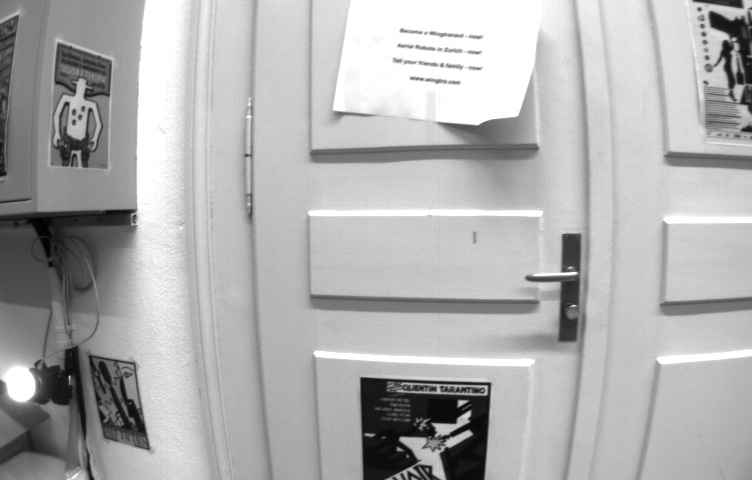
\includegraphics[width=0.75\textwidth]{images/frame0000}
  \caption{Frame from the hand held data set close to the wall}
  \label{fig:dataset_close}
\end{figure}

\begin{figure}[H]
  \centering
  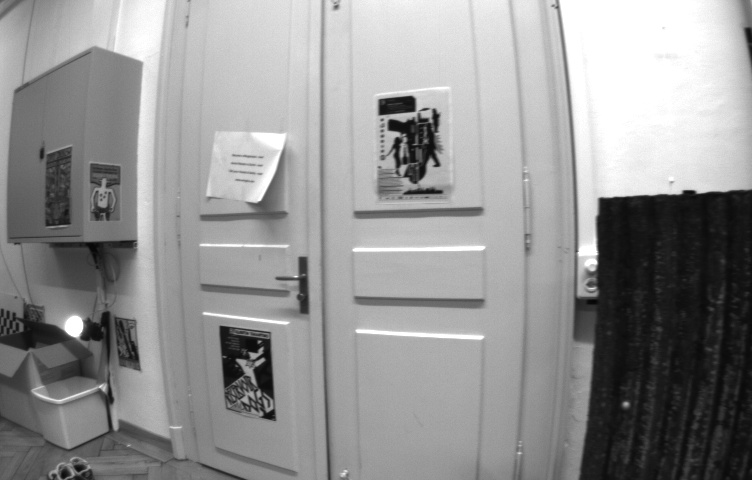
\includegraphics[width=0.75\textwidth]{images/frame0014}
  \caption{Frame from the hand held data set far from the wall}
  \label{fig:dataset_far}
\end{figure}

\subsubsection{\acf{UAV}}
The \ac{UAV} used to record this data set (vi\_loops\_uav) is shown in \autoref{fig:uav}. In this data set loops were flown while the camera of the \ac{UAV} was facing the wall. A frame of the recorded data set is shown in \autoref{fig:dataset_uav}.

\begin{figure}[H]
  \centering
  \includegraphics[width=0.75\textwidth]{images/uav}
  \caption{The used \ac{UAV}}
  \label{fig:uav}
\end{figure}

\begin{figure}[H]
  \centering
  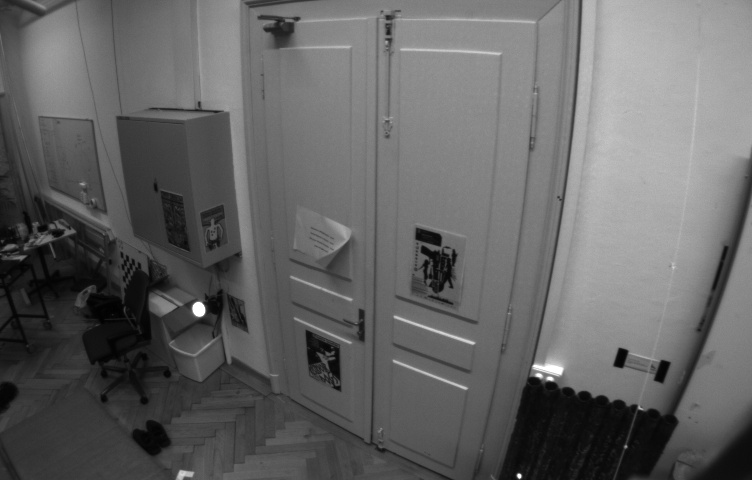
\includegraphics[width=0.75\textwidth]{images/frame0128}
  \caption{Frame from the \ac{UAV} data set}
  \label{fig:dataset_uav}
\end{figure}

\subsection{\acf{ROS} setup}
As already mentioned, the data sets for the two clients were created by splitting a bigger data set recorded with only one client. Because the split data sets don't have the same timing, a re-timing \ac{ROS} node, explained in the next subsection, was written to work around this issue.\\
To get the ground truth in a usable format, a record \ac{ROS} node, explained shortly, was written, which receives the ground truth position from the re-timing \ac{ROS} node and writes it into a text file.\\

The whole \ac{ROS} setup is illustrated in \autoref{fig:ros_setup}.

\tikzstyle{block} = [draw, fill=white, rectangle, minimum height=3em, minimum width=6em]
\tikzstyle{point} = [coordinate]
\begin{figure}[H]
  \centering
  \begin{tikzpicture}[auto, node distance=2cm,>=latex']
		\node [block] (client_1) {rosbag for client 1};
		\node [point] (p1) [right= 1.0cm of client_1]{};
		\node [point] (p2) [below= 0.55cm of p1]{};
		
		\node [block] (client_2) [below = 1.5cm of client_1.west, anchor=west] {rosbag for client 2};	
		\node [point] (p3) [right = 1.0cm of client_2]{};
		\node [point] (p4) [above = 0.5cm of p3]{};
		
		\node [block] (retiming) [below right =-0.3cm and 2cm of client_1] {retiming node};
    \node [point] (p5) [right = 1cm of retiming, yshift=0.2cm]{};
    \node [point] (p7) [above = 0.9cm of p5]{};
    \node [point] (p6) [right = 1cm of retiming, yshift=-0.2cm]{};
    \node [point] (p8) [below = 0.9cm of p6]{};

    \node [block] (slam) [above right = 0.001cm and 2cm of retiming] {SLAM System};
    \node [block] (recording) [below right = 0.001cm and 2cm of retiming] {recording node};
		
		%\draw [-] (publish_image) -- node[name=u] {/cam0/image\_raw, /camera\_imu/vrpn\_client/estimated\_transform} (p1);
		%\draw [-] (publish_image) -- node[name=u] {grayscale images, ground truth positions} (p1);
		\draw [-] (client_1) -- node[name=u] {} (p1);
		\draw [-] (p1) -- (p2);
		\draw [-] (p3) -- (p4);
		
		\draw [-] (client_2) -- (p3);
		
		\draw [->] (p2) -- (p2-|retiming.west);
		\draw [->] (p4) -- (p4-|retiming.west);

    \draw [-] ([yshift=0.2cm]retiming.east) -- (p5);
    \draw [-] ([yshift=-0.2cm]retiming.east) -- (p6);

    \draw [-] (p5) -- (p7);
    \draw [-] (p6) -- (p8);

    \draw [->] (p7) -- (p7-|slam.west);
    \draw [->] (p8) -- (p8-|recording.west);
	\end{tikzpicture}
  \caption{\ac{ROS} setup}
  \label{fig:ros_setup}
\end{figure}

\subsubsection{Re-timing node}
The re-timing \ac{ROS} node subscribes to the topics providing the ground truth position and the greyscale image and republishes the messages of these topics with the time stamp set to the current system time.

\subsubsection{Recording node}
\label{subsubsec:record_node}
The recording \ac{ROS} node subscribes to the topic, which contains the re-timed ground truth position. It saves the ground truth positions into a list and at the end writes all the positions together with their time stamps into a text file.

\subsection{Evaluation}
To evaluate the proposed new map fusion approach and to measure the influence of the culling as well as the change of the optimization algorithm to the accuracy, an evaluation procedure was developed. The evaluation procedure performs the following steps:

\begin{enumerate}
  \item Load ground truth and \ac{SLAM} positions
  \item Find corresponding (in time) ground truth and \ac{SLAM} positions
  \item Perform a 7DoF alignment between the ground truth and the \ac{SLAM} positions
  \item Calculate the \acf{RMSE} between the ground truth and the \ac{SLAM} positions
\end{enumerate}

In the following subsections each step will be described in more detail.

\subsubsection{Loading of the ground truth and \ac{SLAM} positions}
This step involves the loading of the positions from text files, applying the time offset $t_{\text{off}}$ and applying the camera-to-marker transformation $T_{\text{camera\_marker}}$.\\

The offset $t_{\text{off}}$ has to be applied as there is a time offset, emerging from the fact that the \ac{ROS} messages with the greyscale image and the \ac{ROS} messages with the ground truth position do not have the same time of travel, which has to be compensated.\\
For the vi\_loops\_uav data set the time offset varies a lot as both topics are received over a unreliable wireless LAN connection. To counteract this situation different time offsets are tried by brute-forcing and the time offset which results in the smallest \ac{RMSE} is taken.\\ 

As the camera and the marker of the motion tracking system do not have the same position, the transformation $T_{\text{camera\_marker}}$ has to be applied that the ground truth positions and the \ac{SLAM} positions are in the same coordinate system for the evaluation.

\subsubsection{Find corresponding ground truth and \ac{SLAM} positions}
In this step, for every \ac{SLAM} position the first ground truth position with a time stamp higher than the one of the \ac{SLAM} position is searched (line \autoref{line:corr1}). After that, the absolute time difference between the time stamp of the \ac{SLAM} position and the time stamp of the ground truth position, right before the one which was found in the previous step, is calculated (line \autoref{line:corr2}). If this absolute time difference is smaller than the specified accuracy, the ground truth and the \ac{SLAM} positions are saved in a new array (lines \autoref{line:corr2}-\autoref{line:corr3}). The full procedure is listed in \autoref{lst:correspond}.

\lstset{language=Python}
\begin{lstlisting}[frame=single, caption=Find corresponding positions in time, label=lst:correspond]
def time_matching(list_gt_x,list_slam_x,gt_coordinates,
                  slam_coordinates,accuracy):

  # Matching of the datasets according to their time stamps
  gt = np.zeros((len(list_gt_x), 4))
  slam = np.zeros((len(list_slam_x), 4))

  pos = 0
  offset = 1
  break_flag = False
  for i in range(len(list_gt_x)):
    for j in range(offset, len(list_slam_x)):
      # value where slam time > gt time
      if gt_coordinates[i,0] < slam_coordinates[j,0]:|\label{line:corr1}|
        # check the one before
        if abs(gt_coordinates[i,0]-slam_coordinates[j-1,0])|\label{line:corr2}||\Suppressnumber|
                                                < accuracy:|\Reactivatenumber{17}|
          gt[pos] = gt_coordinates[i]
          slam[pos] = slam_coordinates[j - 1]|\label{line:corr3}|
          pos = pos + 1
          if pos >= len(slam_coordinates):
            break_flag = True
            break
          offset = j
          continue
    if break_flag==True:
      break

  # Remove empty rows
  slam = slam[~(slam == 0).all(1)]
  gt = gt[~(gt == 0).all(1)]

  return slam, gt
\end{lstlisting}

\subsubsection{Perform a 7DoF alignment}
A 7DoF alignment is necessary as monocular \ac{SLAM} systems, as the one this semester project is based on, doesn't provide a scale and position and rotation of the \ac{SLAM} coordinate system and the one of the ground truth doesn't have to be the same one.\\

To perform the 7DoF alignment an implementation of the algorithm proposed in \cite{Umeyama1991} was used. This algorithm determines the transformation and the scaling which results in the least \ac{RMSE}. With this transformation and scaling, the \ac{SLAM} positions are transformed and scaled accordingly.

\subsubsection{Calculate the \acf{RMSE}}
The \acf{RMSE} between the ground truth and the \ac{SLAM} positions is calculated according to
\begin{equation}
  \text{\ac{RMSE}} = \sqrt{\frac{1}{N - 1} \sum_i^N \big( (x_{\text{SLAM},i} - x_{\text{gt},i})^2 + (y_{\text{SLAM},i} - y_{\text{gt},i})^2 + (z_{\text{SLAM},i} - z_{\text{gt},i})^2\big)}
\end{equation}
where $N$ is the total number of positions, $x_{\text{SLAM},i}$, $y_{\text{SLAM},i}$ and $z_{\text{SLAM},i}$ are the positions of the \ac{SLAM} system and $x_{\text{gt},i}$, $y_{\text{gt},i}$ and $z_{\text{gt},i}$ are the ground truth positions provided by a motion tracking system.

\section{Experiments}
\label{sec:experiments}

In this section, the performed experiments which show the performance of the proposed new map fusion approach, of the culling and of the different optimization algorithm settings are presented.\\

For every experiment, three runs were performed from which an average for the two maps was calculated. These averages as well as the average of the averaged map results are listed for every experiment.

\subsection{Evaluation of suitable settings}
\label{subsec:suitable_settings}
\subsubsection{Description}
With the first data set, the vi\_loops\_close data set, a variety of different settings (number of \acp{KFM} and number of \acp{KF} to skip after a \ac{KFM}) was evaluated to get an idea of the influence of the two parameters and to choose a selection of suitable settings for the other experiments.

\subsubsection{Results}
The results of this experiment are listed in \autoref{tab:res_1}.

\begin{table}[ht!]
	\begin{center}
		\npdecimalsign{.}
		\nprounddigits{4}
		\begin{tabular}{r|r|n{1}{4}|n{1}{4}|n{1}{4}}
			{\# \acp{KFM}} & {\# \acp{KF} skip} & {\ac{RMSE} Map 1 [m]} & {\ac{RMSE} Map 2 [m]} & {\ac{RMSE} Average [m]} \\ \hline
			1 & 0 & 0.499766666666667 & 0.507333333333333 & 0.50355 \\
			3 & 0 & 0.470333333333333 & 0.6175 & 0.543916666666667 \\
			3 & 5 & 0.445266666666667 & 0.6091 & 0.527183333333333 \\
			3 & 10 & 0.400266666666667 & 0.6392 & 0.519733333333333 \\
			3 & 20 & 0.465733333333333 & 0.628033333333333 & 0.546883333333333 \\
			5 & 0 & 0.5424 & 0.65 & 0.5962 \\
			5 & 5 & 0.465333333333333 & 0.523066666666667 & 0.4942 \\
			5 & 10 & 0.4081 & 0.5128 & 0.46045 \\
			5 & 20 & 0.366833333333333 & 0.4907 & 0.428766666666667 \\
			5 & 30 & 0.4094 & 0.445533333333333 & 0.427466666666667 \\
			5 & 40 & 0.312866666666667 & 0.414266666666667 & 0.363566666666667 \\
			7 & 10 & 0.439433333333333 & 0.5149 & 0.477166666666667 \\
			7 & 20 & 0.396566666666667 & 0.531466666666667 & 0.464016666666667 \\
			10 & 5 & 0.460466666666667 & 0.536466666666667 & 0.498466666666667 \\
			10 & 10 & 0.4283 & 0.438533333333333 & 0.433416666666667 \\
			15 & 5 & 0.4329 & 0.4862 & 0.45955 \\
			15 & 10 & 0.44 & 0.510633333333333 & 0.475316666666667 \\
		\end{tabular}
	\end{center}
	\caption{\acp{RMSE} with the vi\_loop\_close data set}
	\label{tab:res_1}
\end{table}

\subsubsection{Discussion}
In \autoref{tab:res_1} one can see, that with only three \acp{KFM} the \ac{RMSE} gets higher. This may result from the fact, that with only three \acp{KFM} not much more information is gained while the computational effort is increased, as the transformation for every \ac{KFM} is calculated and optimized. If this increased computational effort occurs more or less at once, this could lead to short time overload of the system which then results in a higher \ac{RMSE}. The fact that the \ac{RMSE} is decreased if \acp{KF} are skipped, supports this reasoning as with skipped \acp{KF} the increased computational effort is more spread over time because the time between the transformations of the \acp{KFM} are calculated and optimized is increased due to the skipping of \acp{KF}.

The setting with five \acp{KFM} and no \acp{KF} skipped also results in a worse \ac{RMSE} which could be explained with the same reason mentioned before.

The settings with five and more \acp{KFM} and skipped \acp{KF} results in a lower \ac{RMSE} and therefore a higher accuracy compared to the old approach.\\

The selected settings which will also be evaluated in the other experiments are listed in \autoref{tab:dis_settings}.

\begin{table}[ht!]
	\begin{center}
		\begin{tabular}{r|r}
			\# of \acp{KFM} & \# of \acp{KF} skipped  \\ 
			\hline 
			5 & 20 \\ 
			10 & 5 \\ 
			10 & 10 \\ 
		\end{tabular} 
	\end{center}
	\caption{The selected settings}
	\label{tab:dis_settings}
\end{table}

The selected settings may not be the ones performing best on the first data set (vi\_loop\_close) but they are also well suited for other data sets as they e.g. do not skip too many \acp{KF} or do not require too many \acp{KFM} which could lead to no map fusion in data sets with less overlap.\\

\subsection{Proposed map fusion approach}
\subsubsection{Description}
To evaluate the performance of the proposed map fusion approach, the approach was applied to the vi\_loop\_far data set and to the more challenging vi\_loops\_uav data set, with the chosen settings described in \autoref{subsec:suitable_settings}.

\subsubsection{Results}
The results of the experiment with the vi\_loop\_far data set are listed in \autoref{tab:res_2}. In \autoref{tab:res_3} the results of the experiment with the vi\_loops\_uav data set are listed.

\begin{table}[ht!]
	\npdecimalsign{.}
	\nprounddigits{4}
	\begin{tabular}{r|r|n{1}{4}|n{1}{4}|n{1}{4}}
		{\# \acp{KFM}} & {\# \acp{KF} skip} & {\ac{RMSE} Map 1 [m]} & {\ac{RMSE} Map 2 [m]} & {\ac{RMSE} Average [m]} \\ \hline
		1 & 0 & 0.553166666666667 & 0.4617 & 0.507433333333333 \\
		5 & 20 & 0.3373 & 0.353066666666667 & 0.345183333333333 \\
		10 & 5 & 0.377166666666667 & 0.312666666666667 & 0.344916666666667 \\
		10 & 10 & 0.356933333333333 & 0.3429 & 0.349916666666667 \\
	\end{tabular}
	\caption{\acp{RMSE} with the vi\_loop\_far data set}
	\label{tab:res_2}
\end{table}

\begin{table}[ht!]
	\npdecimalsign{.}
	\nprounddigits{4}
	\begin{tabular}{r|r|n{1}{4}|n{1}{4}|n{1}{4}}
		{\# \acp{KFM}} & {\# \acp{KF} skip} & {\ac{RMSE} Map 1 [m]} & {\ac{RMSE} Map 2 [m]} & {\ac{RMSE} Average [m]} \\ \hline
		1 & 0 & 0.114066666666667 & 0.148066666666667 & 0.131066666666667 \\
		5 & 20 & 0.0736 & 0.108733333333333 & 0.091166666666667 \\
		10 & 5 & 0.1129 & 0.134233333333333 & 0.123566666666667 \\
		10 & 10 & 0.0846 & 0.107533333333333 & 0.096066666666667 \\
	\end{tabular}
	\caption{\acp{RMSE} with the vi\_loop\_uav data set}
	\label{tab:res_3}
\end{table}

\subsubsection{Discussion}
In \autoref{tab:res_2} and \autoref{tab:res_3} one can see, that the \acp{RMSE} are also decreased for the selected settings with the data set vi\_loop\_far, respective vi\_loop\_uav.\\

The presented results show therefore, that with the usage of multiple \acp{KFM} and the skipping of \acp{KF}, the \ac{RMSE} can be reduced, respective the accuracy can be increased. The reduced drift and the increased accuracy is visible, when comparing \autoref{fig:drift_1} and \autoref{fig:drift_2}

\begin{figure}[H]
	\centering
	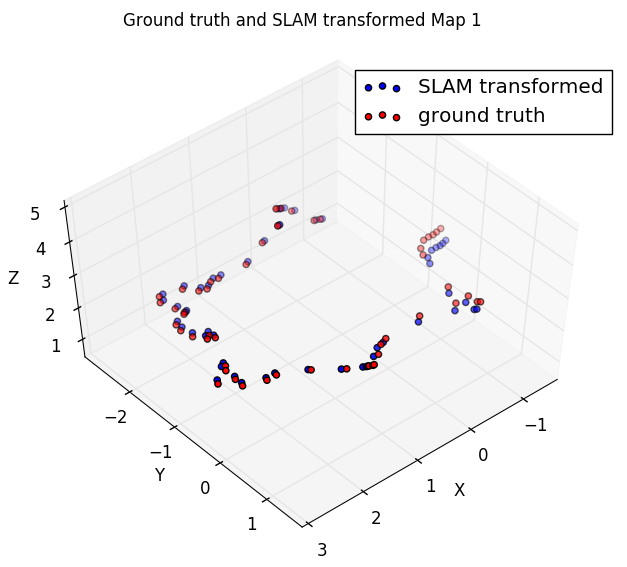
\includegraphics[width=0.75\textwidth]{images/m1_skf0_cut}
	\caption{Drift of a trajectory with the previous approach}
	\label{fig:drift_1}
\end{figure}
\begin{figure}[H]
	\centering
	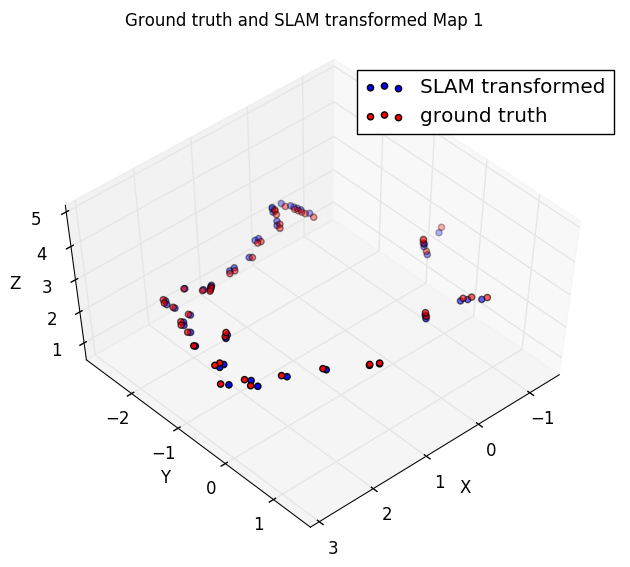
\includegraphics[width=0.75\textwidth]{images/m10_skf10_cut}
	\caption{Drift of a trajectory with the proposed new approach}
	\label{fig:drift_2}
\end{figure}

\subsection{Culling}
\subsubsection{Description}
To determine the influence of the culling, the proposed map fusion approach without and with culling was applied to the vi\_loop\_uav data set. The influence was measured by counting the number of edges and vertices the \ac{PGO} and the \ac{BA} had to process, by measuring the timing of the \ac{PGO} and the \ac{BA} and by calculating the \acp{RMSE}.

\subsubsection{Results}
\autoref{tab:res_4} lists the number of edges and vertices the \ac{PGO} and the \ac{BA} had to process without culling for two representative settings and \autoref{tab:res_5} lists the results with culling.

\begin{table}[ht!]
	\npdecimalsign{.}
	\nprounddigits{0}
	\begin{tabular}{r|r|n{5}{0}|n{5}{0}|n{5}{0}|n{5}{0}}
		{\# \acp{KFM}} & {\# \acp{KF} skip} & {PGO \# edges} & {\ac{PGO} \# verteces} & {\ac{BA} \# edges} & {\ac{BA} \# verteces} \\ \hline
		1 & 0 & 753.666666666667 & 58.6666666666667 & 22193 & 2308 \\
		10 & 10 & 1949.33333333333 & 149.666666666667 & 49765.3333333333 & 4806.33333333333 \\
	\end{tabular}
	\caption{Number of edges and vertices in the \ac{PGO} and in the \ac{BA} without culling with the vi\_loop\_uav data set}
	\label{tab:res_4}
\end{table}

\begin{table}[ht!]
	\npdecimalsign{.}
	\nprounddigits{0}
	\begin{tabular}{r|r|n{5}{0}|n{5}{0}|n{5}{0}|n{5}{0}}
		{\# \acp{KFM}} & {\# \acp{KF} skip} & {PGO \# edges} & {\ac{PGO} \# verteces} & {\ac{BA} \# edges} & {\ac{BA} \# verteces} \\ \hline
		1 & 0 & 282.666666666667 & 35.6666666666667 & 13221.6666666667 & 1892.66666666667 \\
		10 & 10 & 656.666666666667 & 92.6666666666667 & 30453 & 4165 \\
	\end{tabular}
	\caption{Number of edges and vertices in the \ac{PGO} and in the \ac{BA} with culling with the vi\_loop\_uav data set}
	\label{tab:res_5}
\end{table}

The timings of the fusion of \acfp{MP}, the \ac{PGO} and the \ac{BA} without and with culling are listed in \autoref{tab:res_timing_1} and \autoref{tab:res_timing_2}.

\begin{table}[ht!]
	\npdecimalsign{.}
	\nprounddigits{2}
	\begin{center}
		\begin{tabular}{r|r|n{4}{2}|n{4}{2}|n{4}{2}}
			{\# \acp{KFM}} & {\# \acp{KF} skip} & {MPF [ms]} & {\ac{PGO} [ms]} & {\ac{BA} [ms]} \\ \hline
			1 & 0 & 0 & 142.25 & 163.886333333333 \\
			5 & 20 & 44.31 & 649.516666666667 & 2112.18333333333 \\
			10 & 5 & 57.4133333333333 & 372.417666666667 & 1334.04333333333 \\
			10 & 10 & 98.1233333333333 & 532.276666666667 & 3659.48 \\
		\end{tabular}
		\caption{Timings of the MPF, the \ac{PGO} and the \ac{BA} with the vi\_loop\_uav data set without culling}
		\label{tab:res_timing_1}
	\end{center}
\end{table}

\begin{table}[ht!]
	\npdecimalsign{.}
	\nprounddigits{2}
	\begin{center}
		\begin{tabular}{r|r|n{4}{2}|n{4}{2}|n{4}{2}}
			{\# \acp{KFM}} & {\# \acp{KF} skip} & {MPF [ms]} & {\ac{PGO} [ms]} & {\ac{BA} [ms]} \\ \hline
			1 & 0 & 0 & 43.0133333333333 & 72.3266666666667 \\
			5 & 20 & 10.08 & 119.776666666667 & 410.913333333333 \\
			10 & 5 & 16.2366666666667 & 86.09 & 209.413333333333 \\
			10 & 10 & 33.78 & 178.83 & 1098.36666666667 \\
		\end{tabular}
		\caption{Timings of the MPF, the \ac{PGO} and the \ac{BA} with the vi\_loop\_uav data set with culling}
		\label{tab:res_timing_2}
	\end{center}
\end{table}

\autoref{tab:res_6} lists the \acp{RMSE} of the proposed map fusion approach with culling with the vi\_loop\_uav data set.

\begin{table}[ht!]
	\npdecimalsign{.}
	\nprounddigits{4}
	\begin{tabular}{r|r|n{1}{4}|n{1}{4}|n{1}{4}}
		{\# \acp{KFM}} & {\# \acp{KF} skip} & {\ac{RMSE} Map 1 [m]} & {\ac{RMSE} Map 2 [m]} & {\ac{RMSE} Average [m]} \\ \hline
		1 & 0 & 0.199066666666667 & 0.238233333333333 & 0.21865 \\
		5 & 20 & 0.114966666666667 & 0.1315 & 0.123233333333333 \\
		10 & 5 & 0.075033333333333 & 0.088333333333333 & 0.081683333333333 \\
		10 & 10 & 0.083066666666667 & 0.109933333333333 & 0.0965 \\
	\end{tabular}
	\caption{\acp{RMSE} with culling with the vi\_loop\_uav data set}
	\label{tab:res_6}
\end{table}

\subsubsection{Discussion}
With culling, the number of edges and vertices the \ac{PGO} and the \ac{BA} have to process is reduced significantly compared to without culling, as shown in \autoref{tab:res_4} and \autoref{tab:res_5}. The reduction of the number of edges in the \ac{PGO} and in the \ac{BA} is more than 60\%, respectively 38\% and the reduction of the number of vertices in the \ac{PGO} and in the \ac{BA} is up to 38\%, respectively 13\%, as shown in \autoref{tab:res_percentage_1} and \autoref{tab:res_percentage_2}.

\begin{table}[ht!]
	\begin{center}
		\begin{tabular}{r|r|r|r}
			\# \acp{KFM} & \# \acp{KF} skip & \ac{PGO} edges red. [\%] & \ac{PGO} vertices red. [\%]   \\ 
			\hline 
			1 & 0 & 62.47 & 38.98 \\ 
			10 & 10 & 66.29 & 38.00 \\ 
		\end{tabular} 
	\end{center}
	\caption{Reduction of edges and vertices in the \ac{PGO} with culling in percent}
	\label{tab:res_percentage_1}
\end{table}

\begin{table}[ht!]
	\begin{center}
		\begin{tabular}{r|r|r|r}
			\# \acp{KFM} & \# \acp{KF} skip & \ac{BA} edges red. [\%] & \ac{BA} vertices red. [\%]   \\ 
			\hline 
			1 & 0 & 40.42 & 17.98 \\ 
			10 & 10 & 38.81 & 13.34 \\ 
		\end{tabular} 
	\end{center}
	\caption{Reduction of edges and vertices in the \ac{BA} with culling in percent}
	\label{tab:res_percentage_2}
\end{table}

The reduction in edges and vertices then results in a decrease of the runtime as shown in \autoref{tab:res_timing_1} and \autoref{tab:res_timing_2}\\

As the culling removes information, one has to be careful not to remove to many information. With a redundancy threshold of 90\%, the accuracy of the setting with 10 \acp{KFM} and 10 \acp{KF} skipped got worse. Because of this reason, another experiment with a redundancy threshold of 94\% was performed instead, which showed a satisfactory result.\\

With the right choice of the redundancy threshold, the number of edges and vertices in the optimization can be reduced significantly which results in a reduced runtime while achieving the same accuracy.

\subsection{Different optimization algorithms}
\subsubsection{Description}
To compare the performance of the \ac{LM} algorithm with the performance of the \ac{DL} algorithm for the \ac{PGO} and the \ac{BA} in the proposed map fusion approach with culling, the timings and the \acp{RMSE} for all the cases were measured.

\subsubsection{Results}

The timings when the \ac{PGO} and the \ac{BA} both use the \ac{LM} algorithm with the vi\_loop\_uav data set are listed in \autoref{tab:res_timing_2}. In \autoref{tab:res_timing_4}, the timings when the \ac{PGO} and the \ac{BA} both use the \ac{DL} algorithm are listed.

\begin{table}[ht!]
	\npdecimalsign{.}
	\nprounddigits{2}
	\begin{center}
		\begin{tabular}{r|r|n{4}{2}|n{4}{2}|n{4}{2}}
			{\# \acp{KFM}} & {\# \acp{KF} skip} & {MPF [ms]} & {\ac{PGO} [ms]} & {\ac{BA} [ms]} \\ \hline
			1 & 0 & 0 & 48.75 & 68.2433333333333 \\
			5 & 20 & 7.89 & 139.3 & 225.996666666667 \\
		    10 & 5 & 14.2733333333333 & 92.7866666666667 & 164.97 \\			
			10 & 10 & 35.2933333333333 & 243.346666666667 & 446.753333333333 \\
		\end{tabular}
		\caption{Timings of the MPF, the \ac{PGO} and the \ac{BA} both using the \ac{DL} algorithm with the vi\_loop\_uav data set with culling}
		\label{tab:res_timing_4}
	\end{center}
\end{table}

In \autoref{tab:res_6}, the \acp{RMSE} when the \ac{PGO} and the \ac{BA} both use the \ac{LM} algorithm with the vi\_loop\_uav data set are listed. The \acp{RMSE} when the \ac{PGO} and the \ac{BA} both use the \ac{DL} algorithm are listed in \autoref{tab:res_8}.

\begin{table}[ht!]
	\npdecimalsign{.}
	\nprounddigits{4}
	\begin{tabular}{r|r|n{1}{4}|n{1}{4}|n{1}{4}}
		{\# \acp{KFM}} & {\# \acp{KF} skip} & {\ac{RMSE} Map 1 [m]} & {\ac{RMSE} Map 2 [m]} & {\ac{RMSE} Average [m]} \\ \hline
		1 & 0 & 0.1907 & 0.254533333333333 & 0.222616666666667 \\
		5 & 20 & 0.0759 & 0.1099 & 0.0929 \\
		10 & 5 & 0.0656 & 0.089093333333333 & 0.077346666666667 \\
	    10 & 10 & 0.061566666666667 & 0.095233333333333 & 0.0784\\		
	\end{tabular}
	\caption{\acp{RMSE} with \ac{PGO} using the \ac{LM} algorithm and \ac{BA} using the \ac{DL} algorithm with the vi\_loop\_uav data set with culling}
	\label{tab:res_8}
\end{table}

\subsubsection{Discussion}
The timings of both optimization procedures (\ac{PGO} and \ac{BA}) with the \ac{LM} and the \ac{DL} algorithm were recorded and presented in \autoref{tab:res_timing_2} and \autoref{tab:res_timing_4}.

The best results are achieved if for the \ac{PGO} the \ac{LM} algorithm and for the \ac{BA} the \ac{DL} algorithm is used. The timings of this setup are summarized in \autoref{tab:res_timing_6}.

\begin{table}[ht!]
	\npdecimalsign{.}
	\nprounddigits{2}
	\begin{center}
		\begin{tabular}{r|r|n{4}{2}|n{4}{2}|n{4}{2}}
			{\# \acp{KFM}} & {\# \acp{KF} skip} & {MPF [ms]} & {\ac{PGO} [ms]} & {\ac{BA} [ms]} \\ \hline
			1 & 0 & 0 & 43.8266666666667 & 68.7666666666667 \\
			5 & 20 & 6.74 & 99.8033333333333 & 204.363333333333 \\
			10 & 5 & 16 & 93.4466666666667 & 164.576666666667 \\
			10 & 10 & 33.9466666666667 & 178.696666666667 & 383.539666666667 \\
		\end{tabular}
		\caption{Timings of the MPF, the \ac{PGO} and the \ac{BA}, \ac{PGO} using the \ac{LM} algorithm and \ac{BA} using the \ac{DL} algorithm with the vi\_loop\_uav data set with culling}
		\label{tab:res_timing_6}
	\end{center}
\end{table}

That only the \ac{BA} performs better with the \ac{DL} algorithm may come from the fact that the \ac{BA} is a large scale, classically non-linear, optimization problem \cite{Lourakis2005, Triggs2000}, whereas the \ac{PGO} in comparison is a smaller optimization problem, as the \acp{MP} stay fixed and are not optimized, and the \ac{LM} algorithm performs better for smaller optimization problems.\\

With the change of the \ac{BA} using the \ac{DL} algorithm instead of the \ac{LM} algorithm, the runtime of the optimization was decreased and therefore also the runtime of the whole system.\\

%\section{Discussion}